\documentclass[11pt]{article}

\usepackage[margin=0.85in]{geometry}
\usepackage{amsmath,amssymb,bm,mathtools}
\usepackage{booktabs,longtable,array,multirow}
\usepackage{graphicx}
\usepackage{xcolor}
\usepackage{hyperref}
\usepackage{enumitem}
\usepackage{tikz}
\usetikzlibrary{arrows.meta,positioning,shapes.geometric,calc,fit,decorations.pathreplacing}
\usepackage[most]{tcolorbox}
\usepackage{listings}
\usepackage{caption}
\usepackage{float}
\usepackage{microtype}

\hypersetup{
    colorlinks=true,
    linkcolor=blue!60!black,
    citecolor=blue!60!black,
    urlcolor=blue!60!black
}

\definecolor{fluidblue}{RGB}{25,82,140}
\definecolor{fluidgreen}{RGB}{36,135,90}
\definecolor{fluidred}{RGB}{168,54,44}
\definecolor{lightblue}{RGB}{232,242,252}
\definecolor{lightgreen}{RGB}{233,248,239}
\definecolor{lightred}{RGB}{253,238,236}
\definecolor{lightgraybox}{RGB}{246,246,246}
\definecolor{darkgray}{RGB}{60,60,60}

\newcommand{\kn}{\mathrm{Kn}}
\newcommand{\re}{\mathrm{Re}}
\newcommand{\ma}{\mathrm{Ma}}
\newcommand{\mse}{\mathrm{MSE}}
\newcommand{\mae}{\mathrm{MAE}}
\newcommand{\rmse}{\mathrm{RMSE}}
\newcommand{\relL}{\mathrm{Rel}\,L_2}
\newcommand{\R}{\mathbb{R}}
\newcommand{\dd}{\mathrm{d}}
\newcommand{\eps}{\varepsilon}
\newcommand{\btheta}{\bm{\theta}}
\newcommand{\bx}{\bm{x}}
\newcommand{\by}{\bm{y}}
\newcommand{\bwhat}{\widehat{\bm{y}}}
\newcommand{\wh}[1]{\widehat{#1}}

\setlist[itemize]{topsep=3pt,itemsep=2pt,parsep=1pt}
\setlist[enumerate]{topsep=3pt,itemsep=2pt,parsep=1pt}

\tcbset{
  enhanced,
  breakable,
  colback=white,
  colframe=fluidblue!70!black,
  boxrule=0.6pt,
  arc=2pt,
  left=6pt,
  right=6pt,
  top=5pt,
  bottom=5pt
}

\newtcolorbox{keybox}[1]{colback=lightblue,colframe=fluidblue,title=\textbf{#1}}
\newtcolorbox{warnbox}[1]{colback=lightred,colframe=fluidred,title=\textbf{#1}}
\newtcolorbox{examplebox}[1]{colback=lightgreen,colframe=fluidgreen,title=\textbf{#1}}
\newtcolorbox{definitionbox}[1]{colback=lightgraybox,colframe=darkgray,title=\textbf{#1}}

\lstset{
  basicstyle=\ttfamily\small,
  breaklines=true,
  frame=single,
  framerule=0.3pt,
  backgroundcolor=\color{lightgraybox},
  keywordstyle=\color{fluidblue}\bfseries,
  commentstyle=\color{fluidgreen!70!black},
  stringstyle=\color{fluidred!70!black},
  showstringspaces=false,
  tabsize=2
}

\title{\textbf{AI in Fluids -- Week 2}\\[2mm]
Neural Networks for Fluid Surrogates and Rarefied-Flow Variables}
\author{Instructor: Ehsan Roohi\\M\&I-ENG 690A: AI in Fluid Mechanics}
\date{Summer Online Course}

\begin{document}
\maketitle

\begin{center}
\begin{tcolorbox}[width=0.92\linewidth,colback=lightblue,colframe=fluidblue]
\textbf{Course theme:} learn the physics, learn the code, learn from data, and test the limits.\\[2pt]
\textbf{Week 2 theme:} understand what a neural network is, how it makes a prediction, how it learns from data, and how this learning workflow becomes a small rarefied-flow surrogate.
\end{tcolorbox}
\end{center}

\tableofcontents
\newpage

% ============================================================
\section{Purpose of this lecture}

Week 1 built a common starting point: fluid variables, Python arrays, TensorFlow tensors, finite differences, residuals, and the lid-driven cavity benchmark at $\re=100$.  By the end of Week 1, a student should know that a velocity field can be stored as a two-dimensional array, derivatives can be approximated from neighboring grid values, and a numerical result must be validated against a benchmark or a residual.

Week 2 has a different purpose.  It teaches the first real machine-learning model used in the course: a feed-forward neural network.  The main goal is not to memorize software commands.  The goal is to understand the model itself.

\begin{keybox}{Main objective}
By the end of this lecture, a neural network should no longer feel like a black box.  A student should be able to explain:
\begin{itemize}
    \item what the input features are;
    \item what weights and biases do;
    \item how one neuron computes an output;
    \item why activation functions are needed;
    \item how a multi-layer network is built from many neurons;
    \item what a loss function measures;
    \item how gradient descent and backpropagation change weights;
    \item why a low test error is not enough for AI in fluids;
    \item how neural networks become surrogates for rarefied-flow quantities.
\end{itemize}
\end{keybox}

The lecture also introduces the rarefied-flow variables that will be used in the rest of the course: molecular mean free path, Knudsen number, rarefaction regimes, slip, temperature jump, accommodation coefficient, and Knudsen layers.  These variables become features, targets, or validation checks in the coding lab and final projects.

\subsection*{What students should be able to do after Week 2}

After reading this lecture and completing the lab, students should be able to:
\begin{enumerate}
    \item construct a feature matrix $X$ and target array $Y$ from a fluid problem;
    \item distinguish regression from classification;
    \item compute the forward pass of a single neuron by hand;
    \item compute one gradient-descent update for a simple one-neuron model;
    \item describe the roles of weights, biases, activation functions, loss functions, learning rate, batch size, and epochs;
    \item train a small neural network in Python or TensorFlow/Keras;
    \item compare a neural network against a simple baseline;
    \item interpret training and validation curves;
    \item classify continuum, slip, transition, and free-molecular regimes using $\kn$;
    \item explain why extrapolation across rarefaction regimes is dangerous.
\end{enumerate}

\subsection*{How this week fits the six-week course}

\begin{center}
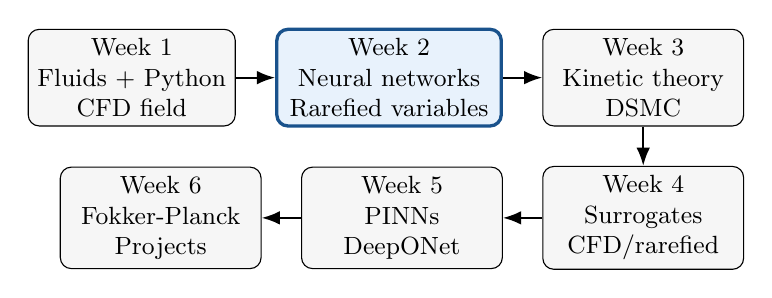
\begin{tikzpicture}[node distance=5mm,>=Latex,every node/.style={font=\small}]
\tikzstyle{week}=[draw,rounded corners,align=center,minimum width=2.55cm,minimum height=1.05cm,fill=lightgraybox]
\tikzstyle{thisweek}=[draw=fluidblue,very thick,rounded corners,align=center,minimum width=2.85cm,minimum height=1.15cm,fill=lightblue]
\node[week] (w1) {Week 1\\Fluids + Python\\CFD field};
\node[thisweek,right=of w1] (w2) {Week 2\\Neural networks\\Rarefied variables};
\node[week,right=of w2] (w3) {Week 3\\Kinetic theory\\DSMC};
\node[week,below=of w3] (w4) {Week 4\\Surrogates\\CFD/rarefied};
\node[week,left=of w4] (w5) {Week 5\\PINNs\\DeepONet};
\node[week,left=of w5] (w6) {Week 6\\Fokker-Planck\\Projects};
\draw[->,thick] (w1)--(w2);
\draw[->,thick] (w2)--(w3);
\draw[->,thick] (w3)--(w4);
\draw[->,thick] (w4)--(w5);
\draw[->,thick] (w5)--(w6);
\end{tikzpicture}
\end{center}

Week 2 is the bridge.  Without it, later topics such as surrogate modeling, PINNs, DeepONet, and neural operators become vocabulary without understanding.

% ============================================================
\section{From a CFD field to a machine-learning dataset}

In Week 1, a two-dimensional incompressible flow field was represented by
\begin{equation}
    u = u(x,y), \qquad v = v(x,y), \qquad p = p(x,y).
    \label{eq:field_continuous}
\end{equation}
Here $x$ and $y$ are spatial coordinates, $u$ is the horizontal velocity component, $v$ is the vertical velocity component, and $p$ is pressure.

On a grid, Eq.~\eqref{eq:field_continuous} becomes
\begin{equation}
    U_{j,i} \approx u(x_i,y_j), \qquad V_{j,i} \approx v(x_i,y_j), \qquad P_{j,i} \approx p(x_i,y_j).
    \label{eq:grid_field}
\end{equation}
Here $i$ is the grid index in the $x$-direction, $j$ is the grid index in the $y$-direction, $x_i$ is the $i$th grid coordinate, $y_j$ is the $j$th grid coordinate, and $U_{j,i}$, $V_{j,i}$, and $P_{j,i}$ are array entries approximating the continuous fields.

A machine-learning dataset can be built by converting each grid location, parameter value, or simulation case into an input-output pair.  A generic supervised-learning dataset is
\begin{equation}
    \mathcal{D}=\left\{\left(\bx^{(i)},\by^{(i)}\right)\right\}_{i=1}^{N}.
    \label{eq:dataset}
\end{equation}
Here $\mathcal{D}$ is the dataset, $N$ is the number of samples, $i$ is the sample index, $\bx^{(i)}\in\mathbb{R}^{d_x}$ is the input feature vector for sample $i$, $d_x$ is the number of input features, $\by^{(i)}\in\mathbb{R}^{d_y}$ is the target vector for sample $i$, and $d_y$ is the number of target quantities.

\begin{definitionbox}{Translation table}
\begin{center}
\begin{tabular}{p{0.26\linewidth}p{0.30\linewidth}p{0.34\linewidth}}
\toprule
Fluid language & Computational language & ML language \\
\midrule
Flow field $u(x,y)$ & 2D array $U_{j,i}$ & Image-like tensor or target field \\
Grid point $(x_i,y_j)$ & Array location $(j,i)$ & Input features $x_i,y_j$ \\
Parameter $\re$ or $\kn$ & Scalar value & Input feature \\
Boundary condition & Array edge values & Constraint or validation check \\
Residual & Equation mismatch & Physics diagnostic or physics loss \\
Benchmark data & Trusted numerical values & Test targets \\
\bottomrule
\end{tabular}
\end{center}
\end{definitionbox}

The neural network does not know what a vortex, shock, or Knudsen layer means unless this information enters through features, targets, physics losses, architecture, or validation.

% ============================================================
\section{Supervised learning: vocabulary and workflow}

Supervised learning means that the model sees examples of inputs and correct outputs.  The model is trained to approximate the mapping from input to output.

\begin{equation}
    \widehat{\by}=f_{\btheta}(\bx).
    \label{eq:model_mapping}
\end{equation}
Here $\bx$ is the input feature vector, $\widehat{\by}$ is the model prediction, $f_{\btheta}$ is the machine-learning model, and $\btheta$ denotes all trainable model parameters, such as neural-network weights and biases.

\begin{definitionbox}{Important terms}
\begin{longtable}{p{0.22\linewidth}p{0.68\linewidth}}
\toprule
Term & Meaning in this course \\
\midrule
Sample & One input-output example, such as one rarefied-flow case or one grid point from one simulation. \\
Feature & An input variable used by the model, such as $\log_{10}\kn$, accommodation coefficient, pressure ratio, or spatial coordinate. \\
Target & The quantity the model should predict, such as mass flow rate, slip velocity, heat flux, density, temperature, or a velocity component. \\
Prediction & The output produced by the model before comparing with the target. \\
Parameter & A trainable number inside the model, usually a weight or bias in a neural network. \\
Loss & A scalar number measuring prediction error on training data. \\
Optimizer & An algorithm that changes model parameters to reduce the loss. \\
Epoch & One pass through the training dataset. \\
Batch & A subset of training samples used for one parameter update. \\
Generalization & Performance on samples not used directly for parameter updates. \\
\bottomrule
\end{longtable}
\end{definitionbox}

\subsection{Regression and classification}

\textbf{Regression} means that the target is a continuous value.  Examples in fluids include predicting a mass flow rate, heat flux, velocity component, pressure coefficient, shock thickness, or slip velocity.

\textbf{Classification} means that the target is a discrete class.  Examples include classifying a flow regime as continuum, slip, transition, or free molecular.

\begin{center}
\begin{tabular}{p{0.30\linewidth}p{0.28\linewidth}p{0.32\linewidth}}
\toprule
Task & Input features & Target \\
\midrule
Regression: mass-flow surrogate & $\left[\log_{10}\kn,\alpha,\Pi,\Theta\right]$ & $Q^*$, normalized mass-flow proxy \\
Regression: pointwise field surrogate & $\left[\re,x,y\right]$ or $\left[\kn,x,y\right]$ & $u$, $v$, $T$, or $\rho$ \\
Classification: rarefaction regime & $\left[\log_{10}\kn\right]$ & continuum/slip/transition/free molecular \\
Classification: model choice & local $\kn$, gradient $\kn$, $\ma$ & continuum solver / kinetic solver / hybrid solver \\
\bottomrule
\end{tabular}
\end{center}

In the first row, $\alpha$ is the gas-surface accommodation coefficient, $\Pi$ is a pressure ratio, $\Theta$ is a wall-temperature ratio, and $Q^*$ is a nondimensional mass-flow proxy.

% ============================================================
\section{A first analogy: a linear decision rule}

A common teaching starting point for neural networks is a two-feature decision problem.  Instead of using a non-fluid example, we use a simple rarefied-flow classification example.

Suppose we want to classify a case as ``continuum-like'' or ``rarefied'' using two features:
\begin{equation}
    x_1 = \log_{10}(\kn), \qquad x_2 = \alpha.
    \label{eq:two_features}
\end{equation}
Here $x_1$ is the base-10 logarithm of the Knudsen number, $\kn$ is the Knudsen number, $x_2$ is the accommodation coefficient, and $\alpha$ measures gas-surface accommodation.

A very simple model is
\begin{equation}
    z = w_1 x_1 + w_2 x_2 + b.
    \label{eq:linear_score}
\end{equation}
Here $z$ is the pre-activation score, $w_1$ and $w_2$ are weights multiplying the two features, and $b$ is the bias.  The score $z$ is then passed through a step function:
\begin{equation}
    o = H(z)=
    \begin{cases}
    1, & z\ge 0,\\
    0, & z<0.
    \end{cases}
    \label{eq:step_output}
\end{equation}
Here $o$ is the model output and $H(z)$ is the Heaviside step activation.  The output $o=1$ could mean ``rarefied'' and $o=0$ could mean ``continuum-like.''

The boundary between the two classes is
\begin{equation}
    w_1x_1+w_2x_2+b=0.
    \label{eq:decision_boundary}
\end{equation}
Here $w_1$, $w_2$, and $b$ are the same parameters used in Eq.~\eqref{eq:linear_score}, and $x_1$ and $x_2$ are the features defined in Eq.~\eqref{eq:two_features}.  This equation is a line in the two-dimensional feature plane.

\begin{center}
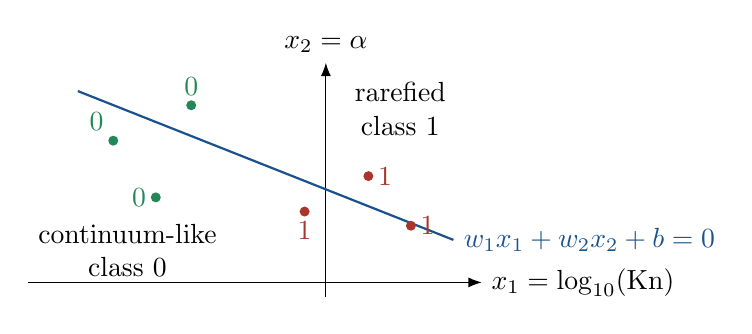
\begin{tikzpicture}[scale=0.9,>=Latex]
\draw[->] (-4.2,0) -- (2.2,0) node[right] {$x_1=\log_{10}(\kn)$};
\draw[->] (0,-0.2) -- (0,3.1) node[above] {$x_2=\alpha$};
\draw[thick,fluidblue] (-3.5,2.7) -- (1.8,0.6) node[right] {$w_1x_1+w_2x_2+b=0$};
\fill[fluidgreen] (-3,2.0) circle (2pt) node[above left] {0};
\fill[fluidgreen] (-2.4,1.2) circle (2pt) node[left] {0};
\fill[fluidgreen] (-1.9,2.5) circle (2pt) node[above] {0};
\fill[fluidred] (-0.3,1.0) circle (2pt) node[below] {1};
\fill[fluidred] (0.6,1.5) circle (2pt) node[right] {1};
\fill[fluidred] (1.2,0.8) circle (2pt) node[right] {1};
\node[align=center] at (-2.8,0.45) {continuum-like\\class 0};
\node[align=center] at (1.05,2.45) {rarefied\\class 1};
\end{tikzpicture}
\end{center}

This is the first important idea: a neuron with a step activation draws a boundary in feature space.  Learning means changing $w_1$, $w_2$, and $b$ until that boundary separates the training examples as well as possible.

% ============================================================
\section{The artificial neuron}

A single artificial neuron takes several input features, multiplies them by weights, adds a bias, and then applies an activation function.

\begin{equation}
    z = \sum_{j=1}^{m} w_j x_j + b = \bm{w}^{T}\bx+b.
    \label{eq:neuron_z}
\end{equation}
Here $m$ is the number of input features, $j$ is the feature index, $x_j$ is the $j$th input feature, $w_j$ is the weight multiplying $x_j$, $b$ is the bias, $\bx=[x_1,x_2,\ldots,x_m]^T$ is the feature vector, $\bm{w}=[w_1,w_2,\ldots,w_m]^T$ is the weight vector, $T$ denotes transpose, and $z$ is the pre-activation value.

The neuron output is
\begin{equation}
    o = \phi(z).
    \label{eq:neuron_o}
\end{equation}
Here $o$ is the neuron output and $\phi$ is the activation function.  The activation function may be a step function, sigmoid, hyperbolic tangent, ReLU, ELU, or a linear function.

\begin{center}
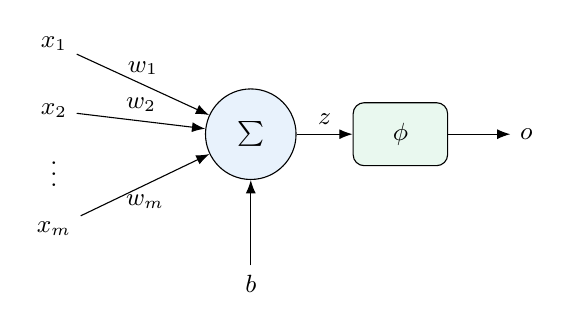
\begin{tikzpicture}[>=Latex,node distance=1.0cm,every node/.style={font=\small}]
\node (x1) at (0,1.3) {$x_1$};
\node (x2) at (0,0.45) {$x_2$};
\node (xd) at (0,-0.25) {$\vdots$};
\node (xm) at (0,-1.05) {$x_m$};
\node[circle,draw,minimum size=1.15cm,fill=lightblue] (sum) at (2.5,0.15) {$\sum$};
\node[rectangle,draw,rounded corners,minimum width=1.2cm,minimum height=0.8cm,fill=lightgreen] (act) at (4.4,0.15) {$\phi$};
\node (out) at (6.0,0.15) {$o$};
\draw[->] (x1) -- node[above] {$w_1$} (sum);
\draw[->] (x2) -- node[above] {$w_2$} (sum);
\draw[->] (xm) -- node[below] {$w_m$} (sum);
\node (b) at (2.5,-1.75) {$b$};
\draw[->] (b) -- (sum);
\draw[->] (sum) -- node[above] {$z$} (act);
\draw[->] (act) -- (out);
\end{tikzpicture}
\end{center}

\subsection{Physical interpretation of weights and bias}

Weights tell the model how strongly each feature affects the prediction.  A large positive weight means that increasing the feature tends to increase the pre-activation value $z$.  A large negative weight means that increasing the feature tends to decrease $z$.  A weight close to zero means that the feature has little direct influence in that neuron.

The bias shifts the neuron threshold.  Without $b$, the boundary $\bm{w}^T\bx=0$ must pass through the origin of feature space.  With $b$, the boundary can move.

\begin{examplebox}{Fluid example}
If $x_1=\log_{10}\kn$ has a positive weight in a neuron predicting rarefaction strength, increasing $\kn$ tends to increase that neuron's output.  If $x_2=\alpha$ has a negative weight, increasing accommodation may reduce that neuron's contribution to the predicted slip correction.  The final behavior of a multi-layer network is more complicated, but this single-neuron interpretation is a useful starting point.
\end{examplebox}

% ============================================================
\section{Activation functions}

If every neuron used only a linear operation, a deep neural network would collapse into one linear mapping.  Activation functions introduce nonlinearity.  Nonlinearity is essential because fluid relations are usually nonlinear: vortices, shocks, slip, temperature jump, Knudsen layers, and transition-regime effects are not linear functions of the input parameters.

\begin{longtable}{p{0.22\linewidth}p{0.30\linewidth}p{0.38\linewidth}}
\toprule
Activation & Formula & Common use \\
\midrule
Step & $\phi(z)=0$ if $z<0$, $\phi(z)=1$ if $z\ge0$ & Simple perceptron classification; not convenient for gradient training because derivative is zero almost everywhere. \\
Sigmoid & $\phi(z)=\dfrac{1}{1+e^{-z}}$ & Binary classification output or probability-like value. \\
Tanh & $\phi(z)=\tanh(z)$ & Hidden layers when outputs centered near zero are helpful. \\
ReLU & $\phi(z)=\max(0,z)$ & Common hidden-layer activation in deep networks. \\
ELU & $\phi(z)=z$ for $z\ge0$, $\phi(z)=a(e^z-1)$ for $z<0$ & Hidden layers; smoother negative branch than ReLU. \\
Linear & $\phi(z)=z$ & Regression output layer when target can be any real value. \\
\bottomrule
\end{longtable}

In the table, $z$ is the pre-activation scalar defined in Eq.~\eqref{eq:neuron_z}, $e$ is the base of the natural logarithm, $a>0$ is a chosen ELU shape parameter, and $\phi(z)$ is the activation output.

\subsection{Derivatives of common activations}

Backpropagation uses activation derivatives.  For example,
\begin{equation}
    \frac{\dd}{\dd z}\left[\frac{1}{1+e^{-z}}\right]
    = \sigma(z)\left[1-\sigma(z)\right],
    \label{eq:sigmoid_derivative}
\end{equation}
where $z$ is the scalar input, $\sigma(z)=1/(1+e^{-z})$ is the sigmoid function, $e$ is the base of the natural logarithm, and $\dd/\dd z$ denotes differentiation with respect to $z$.

For ReLU,
\begin{equation}
    \frac{\dd}{\dd z}\max(0,z)=
    \begin{cases}
    0, & z<0,\\
    1, & z>0.
    \end{cases}
    \label{eq:relu_derivative}
\end{equation}
Here $z$ is the scalar input.  The derivative at $z=0$ is not unique; in software it is assigned a convenient value, often zero.

% ============================================================
\section{Targets, predictions, errors, and loss functions}

For one supervised-learning sample, let the target be $t$ and the prediction be $o$.  The prediction error is
\begin{equation}
    e = t-o.
    \label{eq:error_one}
\end{equation}
Here $e$ is the scalar prediction error, $t$ is the true target value, and $o$ is the model output.

A common one-sample squared-error loss is
\begin{equation}
    C = \frac{1}{2}(t-o)^2.
    \label{eq:single_loss}
\end{equation}
Here $C$ is the cost or loss for one sample, $t$ is the target, and $o$ is the prediction.  The factor $1/2$ is included because it cancels the factor of $2$ that appears when differentiating the square.

For $N$ samples, the mean-squared error is
\begin{equation}
    \mse = \frac{1}{N}\sum_{i=1}^{N}\left(y^{(i)}-\widehat{y}^{(i)}\right)^2.
    \label{eq:mse_scalar}
\end{equation}
Here $N$ is the number of samples, $i$ is the sample index, $y^{(i)}$ is the true scalar target for sample $i$, $\widehat{y}^{(i)}$ is the predicted scalar target for sample $i$, and $\mse$ is the mean-squared error.

The root-mean-squared error is
\begin{equation}
    \rmse = \sqrt{\frac{1}{N}\sum_{i=1}^{N}\left(y^{(i)}-\widehat{y}^{(i)}\right)^2}.
    \label{eq:rmse_scalar}
\end{equation}
Here $\rmse$ has the same units as the target quantity, while $N$, $i$, $y^{(i)}$, and $\widehat{y}^{(i)}$ are defined as in Eq.~\eqref{eq:mse_scalar}.

For a predicted field, a relative $L_2$ error is often useful:
\begin{equation}
    \relL = \frac{\left\|\by-\widehat{\by}\right\|_2}{\left\|\by\right\|_2}.
    \label{eq:rel_l2}
\end{equation}
Here $\by$ is the vector of true field values, $\widehat{\by}$ is the vector of predicted field values, $\|\cdot\|_2$ is the Euclidean norm, and $\relL$ is the relative $L_2$ error.

\begin{warnbox}{Low loss is not enough}
A neural-network surrogate can have a small average error but still violate physics.  In fluids, always ask additional questions: Is density positive?  Does the wall behavior make sense?  Is mass conserved?  Is the shock location correct?  Is the prediction being made outside the training regime?
\end{warnbox}

% ============================================================
\section{Learning: how one neuron changes its weights}

Learning means changing the trainable parameters to reduce the loss.  In a one-neuron model, the trainable parameters are the weights and the bias.

For a linear-output neuron,
\begin{equation}
    o = z = \sum_{j=1}^{m} w_jx_j+b.
    \label{eq:linear_neuron_output}
\end{equation}
Here $o$ is the scalar output, $z$ is the pre-activation value, $m$ is the number of features, $x_j$ is the $j$th feature, $w_j$ is the $j$th weight, and $b$ is the bias.

Using the one-sample loss in Eq.~\eqref{eq:single_loss}, the derivative of $C$ with respect to weight $w_j$ is
\begin{equation}
    \frac{\partial C}{\partial w_j} = -(t-o)x_j.
    \label{eq:grad_w_linear}
\end{equation}
Here $\partial C/\partial w_j$ is the gradient of the loss with respect to weight $w_j$, $C$ is the one-sample loss, $t$ is the target, $o$ is the model output, and $x_j$ is the $j$th input feature.

The derivative of $C$ with respect to the bias is
\begin{equation}
    \frac{\partial C}{\partial b} = -(t-o).
    \label{eq:grad_b_linear}
\end{equation}
Here $\partial C/\partial b$ is the gradient of the loss with respect to bias $b$, and $t-o$ is the prediction error defined in Eq.~\eqref{eq:error_one}.

Gradient descent updates the weight using
\begin{equation}
    w_j \leftarrow w_j - \eta\frac{\partial C}{\partial w_j}.
    \label{eq:gd_w}
\end{equation}
Here $w_j$ is the weight being updated, $\eta>0$ is the learning rate, $C$ is the loss, and $\partial C/\partial w_j$ is the gradient.

The bias update is
\begin{equation}
    b \leftarrow b - \eta\frac{\partial C}{\partial b}.
    \label{eq:gd_b}
\end{equation}
Here $b$ is the bias, $\eta$ is the learning rate, and $\partial C/\partial b$ is the gradient with respect to $b$.

Using Eqs.~\eqref{eq:grad_w_linear} and \eqref{eq:grad_b_linear}, the updates become
\begin{equation}
    w_j \leftarrow w_j + \eta(t-o)x_j, \qquad b \leftarrow b + \eta(t-o).
    \label{eq:perceptron_like_update}
\end{equation}
Here $w_j$ is the $j$th weight, $b$ is the bias, $\eta$ is the learning rate, $t$ is the target, $o$ is the prediction, and $x_j$ is the $j$th feature.

\subsection{Worked numerical example}

Consider a one-neuron surrogate that predicts a normalized rarefied mass-flow correction $Q^*$ from two features:
\begin{equation}
    x_1 = \log_{10}(\kn), \qquad x_2 = \alpha.
    \label{eq:example_features}
\end{equation}
Here $x_1$ is the logarithmic Knudsen-number feature, $\kn$ is the Knudsen number, $x_2$ is the accommodation coefficient, and $\alpha$ measures gas-surface accommodation.

Use the linear-output neuron
\begin{equation}
    o = w_1x_1+w_2x_2+b.
    \label{eq:example_output}
\end{equation}
Here $o$ is the predicted normalized correction, $w_1$ and $w_2$ are weights, $x_1$ and $x_2$ are features, and $b$ is the bias.

Take one training sample:
\begin{equation}
    x_1=-2, \qquad x_2=0.8, \qquad t=0.25.
    \label{eq:example_sample}
\end{equation}
Here $x_1=-2$ corresponds to $\kn=10^{-2}$, $x_2=0.8$ is the accommodation coefficient, and $t=0.25$ is the target normalized correction.

Start with
\begin{equation}
    w_1=0.20, \qquad w_2=-0.10, \qquad b=0.05.
    \label{eq:example_initial}
\end{equation}
Here $w_1$ and $w_2$ are initial weights and $b$ is the initial bias.

The prediction is
\begin{equation}
    o=(0.20)(-2)+(-0.10)(0.8)+0.05=-0.43.
    \label{eq:example_prediction}
\end{equation}
Here $o$ is the model output computed from Eq.~\eqref{eq:example_output} using the values in Eqs.~\eqref{eq:example_sample} and \eqref{eq:example_initial}.

The error is
\begin{equation}
    e=t-o=0.25-(-0.43)=0.68.
    \label{eq:example_error}
\end{equation}
Here $e$ is the prediction error, $t=0.25$ is the target, and $o=-0.43$ is the prediction.

Choose learning rate
\begin{equation}
    \eta=0.05.
    \label{eq:example_eta}
\end{equation}
Here $\eta$ is the learning rate controlling the update size.

Using Eq.~\eqref{eq:perceptron_like_update}, the new weights are
\begin{align}
    w_1^{\rm new} &= 0.20 + (0.05)(0.68)(-2)=0.132, \label{eq:example_w1new}\\
    w_2^{\rm new} &= -0.10 + (0.05)(0.68)(0.8)=-0.0728, \label{eq:example_w2new}\\
    b^{\rm new} &= 0.05 + (0.05)(0.68)=0.084. \label{eq:example_bnew}
\end{align}
Here $w_1^{\rm new}$ and $w_2^{\rm new}$ are the updated weights, $b^{\rm new}$ is the updated bias, $\eta=0.05$ is the learning rate, and $0.68$ is the prediction error from Eq.~\eqref{eq:example_error}.

The new prediction is
\begin{equation}
    o^{\rm new}=(0.132)(-2)+(-0.0728)(0.8)+0.084=-0.23824.
    \label{eq:example_new_prediction}
\end{equation}
Here $o^{\rm new}$ is the prediction after one update.  It is still far from $t=0.25$, but it moved in the correct direction: from $-0.43$ to $-0.23824$.

This example shows what training does.  Training is repeated many times over many samples until the model parameters produce acceptable predictions.

% ============================================================
\section{Learning rate, instability, and slow learning}

The learning rate $\eta$ in Eqs.~\eqref{eq:gd_w} and \eqref{eq:gd_b} controls how large each update is.

\begin{itemize}
    \item If $\eta$ is too small, the loss decreases very slowly.
    \item If $\eta$ is too large, the loss may oscillate or diverge.
    \item If $\eta$ is reasonable, the loss usually decreases over training.
\end{itemize}

\begin{center}
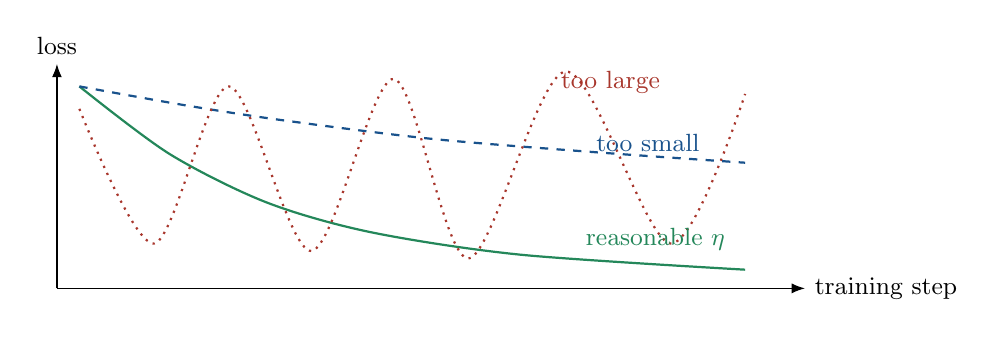
\begin{tikzpicture}[scale=0.95,>=Latex,every node/.style={font=\small}]
\draw[->] (0,0) -- (10,0) node[right] {training step};
\draw[->] (0,0) -- (0,3.0) node[above] {loss};
\draw[fluidgreen,thick] plot[smooth] coordinates {(0.3,2.7) (1.5,1.8) (2.8,1.15) (4.2,0.75) (6.2,0.45) (9.2,0.25)};
\draw[fluidblue,thick,dashed] plot[smooth] coordinates {(0.3,2.7) (1.7,2.45) (3.0,2.25) (5.0,2.0) (7.2,1.82) (9.2,1.68)};
\draw[fluidred,thick,dotted] plot[smooth] coordinates {(0.3,2.4) (1.3,0.6) (2.3,2.7) (3.4,0.5) (4.5,2.8) (5.5,0.4) (6.8,2.9) (8.2,0.6) (9.2,2.6)};
\node[fluidgreen] at (8.0,0.65) {reasonable $\eta$};
\node[fluidblue] at (7.9,1.95) {too small};
\node[fluidred] at (7.4,2.75) {too large};
\end{tikzpicture}
\end{center}

Here $\eta$ is the learning rate, and ``loss'' is the training objective such as MSE.

% ============================================================
\section{From one neuron to a multi-layer perceptron}

One neuron can only create a simple linear boundary or a simple regression formula.  Real fluid relations are usually more complex.  A multi-layer perceptron, or MLP, combines many neurons into layers.

Let the input layer be
\begin{equation}
    \bm{a}^{(0)}=\bx.
    \label{eq:input_layer}
\end{equation}
Here $\bm{a}^{(0)}$ is the activation vector of layer $0$, and $\bx$ is the input feature vector.

For layer $\ell$, the pre-activation vector is
\begin{equation}
    \bm{z}^{(\ell)} = W^{(\ell)}\bm{a}^{(\ell-1)}+\bm{b}^{(\ell)}.
    \label{eq:layer_z}
\end{equation}
Here $\ell$ is the layer index, $\bm{z}^{(\ell)}$ is the pre-activation vector in layer $\ell$, $W^{(\ell)}$ is the weight matrix of layer $\ell$, $\bm{a}^{(\ell-1)}$ is the activation vector from the previous layer, and $\bm{b}^{(\ell)}$ is the bias vector of layer $\ell$.

The activation vector is
\begin{equation}
    \bm{a}^{(\ell)} = \phi^{(\ell)}\left(\bm{z}^{(\ell)}\right).
    \label{eq:layer_a}
\end{equation}
Here $\bm{a}^{(\ell)}$ is the activation vector in layer $\ell$, $\phi^{(\ell)}$ is the activation function for layer $\ell$, and $\bm{z}^{(\ell)}$ is defined in Eq.~\eqref{eq:layer_z}.  The activation is applied component by component.

For a network with $L$ layers, the prediction is
\begin{equation}
    \widehat{\by} = \bm{a}^{(L)}.
    \label{eq:network_output}
\end{equation}
Here $\widehat{\by}$ is the model prediction, $L$ is the index of the output layer, and $\bm{a}^{(L)}$ is the activation vector of the output layer.

\begin{center}
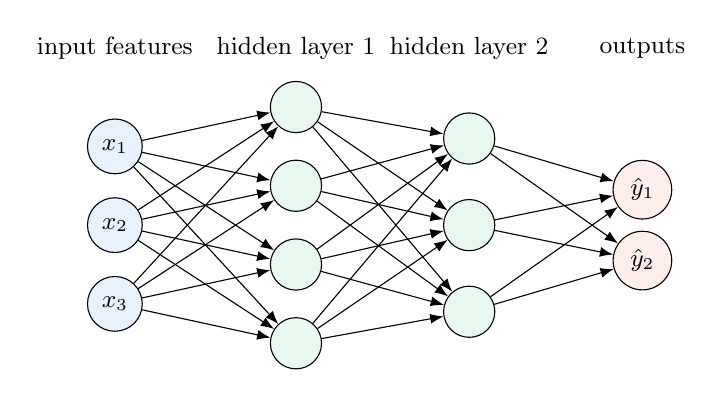
\begin{tikzpicture}[>=Latex,node distance=1cm,every node/.style={font=\small}]
\tikzstyle{neuron}=[circle,draw,minimum size=6.5mm,fill=white]
\node[neuron,fill=lightblue] (x1) at (0,1) {$x_1$};
\node[neuron,fill=lightblue] (x2) at (0,0) {$x_2$};
\node[neuron,fill=lightblue] (x3) at (0,-1) {$x_3$};
\foreach \i/\y in {1/1.5,2/0.5,3/-0.5,4/-1.5}{\node[neuron,fill=lightgreen] (h1\i) at (2.3,\y) {};}
\foreach \i/\y in {1/1.1,2/0.0,3/-1.1}{\node[neuron,fill=lightgreen] (h2\i) at (4.5,\y) {};}
\node[neuron,fill=lightred] (y1) at (6.7,0.45) {$\hat y_1$};
\node[neuron,fill=lightred] (y2) at (6.7,-0.45) {$\hat y_2$};
\foreach \a in {x1,x2,x3}{\foreach \b in {h11,h12,h13,h14}{\draw[->,thin] (\a)--(\b);}}
\foreach \a in {h11,h12,h13,h14}{\foreach \b in {h21,h22,h23}{\draw[->,thin] (\a)--(\b);}}
\foreach \a in {h21,h22,h23}{\foreach \b in {y1,y2}{\draw[->,thin] (\a)--(\b);}}
\node at (0,2.25) {input features};
\node at (2.3,2.25) {hidden layer 1};
\node at (4.5,2.25) {hidden layer 2};
\node at (6.7,2.25) {outputs};
\end{tikzpicture}
\end{center}

\subsection{Why hidden layers help}

Each hidden neuron creates a transformed feature.  The next layer combines those transformed features.  With enough neurons and nonlinear activations, an MLP can approximate complicated nonlinear functions.  This is why MLPs are used for regression surrogates.

For example, a rarefied-flow surrogate may approximate
\begin{equation}
    Q^* \approx f_{\btheta}\left(\log_{10}\kn,\alpha,\Pi,\Theta\right).
    \label{eq:q_surrogate_basic}
\end{equation}
Here $Q^*$ is a nondimensional mass-flow proxy, $f_{\btheta}$ is the neural-network model, $\btheta$ denotes all trainable weights and biases, $\kn$ is Knudsen number, $\alpha$ is accommodation coefficient, $\Pi$ is pressure ratio, and $\Theta$ is wall-temperature ratio.

% ============================================================
\section{Backpropagation: how deep networks learn}

For a one-neuron model, the gradient is easy to write directly.  In a multi-layer network, a weight in an early layer affects the output only through later layers.  Backpropagation is the efficient application of the chain rule to compute all these gradients.

\subsection{Chain rule idea}

If
\begin{equation}
    q = f(g(s)),
    \label{eq:chain_q}
\end{equation}
where $s$ is an input variable, $g$ is an intermediate function, $f$ is an outer function, and $q$ is the final output, then
\begin{equation}
    \frac{\dd q}{\dd s}=\frac{\dd f}{\dd g}\frac{\dd g}{\dd s}.
    \label{eq:chain_rule}
\end{equation}
Here $\dd q/\dd s$ is the derivative of the output with respect to $s$, $\dd f/\dd g$ is the derivative of the outer function with respect to its input $g$, and $\dd g/\dd s$ is the derivative of the intermediate function with respect to $s$.

A neural network is a long composition of functions.  Backpropagation applies Eq.~\eqref{eq:chain_rule} from the output layer backward to the earlier layers.

\subsection{Backpropagation formulas for an MLP}

Consider a network with layer equations \eqref{eq:layer_z} and \eqref{eq:layer_a}.  For one training sample, define the squared-error loss
\begin{equation}
    C = \frac{1}{2}\left\|\bm{a}^{(L)}-\by\right\|_2^2.
    \label{eq:bp_loss}
\end{equation}
Here $C$ is the one-sample loss, $\bm{a}^{(L)}$ is the output-layer activation vector, $L$ is the output-layer index, $\by$ is the target vector, and $\|\cdot\|_2$ is the Euclidean norm.

For the output layer, define the error signal
\begin{equation}
    \bm{\delta}^{(L)} = \left(\bm{a}^{(L)}-\by\right)\odot \phi'^{(L)}\left(\bm{z}^{(L)}\right).
    \label{eq:delta_output}
\end{equation}
Here $\bm{\delta}^{(L)}$ is the output-layer error signal, $\bm{a}^{(L)}$ is the prediction vector, $\by$ is the target vector, $\odot$ denotes componentwise multiplication, $\phi'^{(L)}$ is the derivative of the output-layer activation, and $\bm{z}^{(L)}$ is the output-layer pre-activation vector.

For a hidden layer $\ell$, the error signal is
\begin{equation}
    \bm{\delta}^{(\ell)} = \left[(W^{(\ell+1)})^T\bm{\delta}^{(\ell+1)}\right]\odot \phi'^{(\ell)}\left(\bm{z}^{(\ell)}\right).
    \label{eq:delta_hidden}
\end{equation}
Here $\bm{\delta}^{(\ell)}$ is the error signal in hidden layer $\ell$, $W^{(\ell+1)}$ is the weight matrix of the next layer, $T$ denotes transpose, $\bm{\delta}^{(\ell+1)}$ is the next-layer error signal, $\phi'^{(\ell)}$ is the derivative of the activation in layer $\ell$, and $\bm{z}^{(\ell)}$ is the pre-activation vector in layer $\ell$.

The gradients are
\begin{equation}
    \frac{\partial C}{\partial W^{(\ell)}} = \bm{\delta}^{(\ell)}\left(\bm{a}^{(\ell-1)}\right)^T,
    \label{eq:grad_W_layer}
\end{equation}
where $\partial C/\partial W^{(\ell)}$ is the gradient matrix for weights in layer $\ell$, $\bm{\delta}^{(\ell)}$ is the layer-$\ell$ error signal, and $\bm{a}^{(\ell-1)}$ is the activation vector from the previous layer.

The bias gradient is
\begin{equation}
    \frac{\partial C}{\partial \bm{b}^{(\ell)}} = \bm{\delta}^{(\ell)}.
    \label{eq:grad_b_layer}
\end{equation}
Here $\partial C/\partial \bm{b}^{(\ell)}$ is the gradient of the loss with respect to the bias vector in layer $\ell$, and $\bm{\delta}^{(\ell)}$ is the layer error signal.

The gradient-descent updates are
\begin{align}
    W^{(\ell)} &\leftarrow W^{(\ell)} - \eta \frac{\partial C}{\partial W^{(\ell)}}, \label{eq:update_W_layer}\\
    \bm{b}^{(\ell)} &\leftarrow \bm{b}^{(\ell)} - \eta \frac{\partial C}{\partial \bm{b}^{(\ell)}}. \label{eq:update_b_layer}
\end{align}
Here $W^{(\ell)}$ and $\bm{b}^{(\ell)}$ are the trainable weights and biases in layer $\ell$, $\eta$ is the learning rate, and the gradients are defined in Eqs.~\eqref{eq:grad_W_layer} and \eqref{eq:grad_b_layer}.

\begin{keybox}{Backpropagation in words}
Backpropagation asks: if the output is wrong, how much should each weight and bias in every layer be blamed?  The algorithm computes this blame using derivatives, then the optimizer adjusts the parameters to reduce future error.
\end{keybox}

% ============================================================
\section{Stochastic gradient descent, batches, Adam, and momentum}

In real training, we usually do not compute gradients using the entire dataset at every update.  Instead, we use mini-batches.

For a mini-batch $\mathcal{B}$, the batch loss is
\begin{equation}
    C_{\mathcal{B}} = \frac{1}{|\mathcal{B}|}\sum_{i\in\mathcal{B}} C^{(i)}.
    \label{eq:batch_loss}
\end{equation}
Here $\mathcal{B}$ is a set of sample indices in the mini-batch, $|\mathcal{B}|$ is the number of samples in the mini-batch, $i$ is a sample index, $C^{(i)}$ is the loss for sample $i$, and $C_{\mathcal{B}}$ is the average mini-batch loss.

Stochastic gradient descent updates a parameter vector $\btheta$ as
\begin{equation}
    \btheta_{k+1}=\btheta_k-\eta\nabla_{\btheta} C_{\mathcal{B}}(\btheta_k).
    \label{eq:sgd_update}
\end{equation}
Here $\btheta_k$ is the parameter vector at update step $k$, $\btheta_{k+1}$ is the parameter vector after the update, $\eta$ is the learning rate, $\nabla_{\btheta}$ denotes the gradient with respect to $\btheta$, and $C_{\mathcal{B}}$ is the mini-batch loss.

Momentum smooths the update direction:
\begin{align}
    \bm{v}_{k+1} &= \beta \bm{v}_k + (1-\beta)\bm{g}_k, \label{eq:momentum_v}\\
    \btheta_{k+1} &= \btheta_k - \eta \bm{v}_{k+1}. \label{eq:momentum_update}
\end{align}
Here $\bm{v}_k$ is the momentum vector at step $k$, $\beta\in[0,1)$ is the momentum coefficient, $\bm{g}_k=\nabla_{\btheta}C_{\mathcal{B}}(\btheta_k)$ is the current gradient, $\eta$ is the learning rate, and $\btheta_k$ is the parameter vector.

Adam is a popular optimizer that combines ideas from momentum and adaptive learning rates.  In this course, students do not need to derive Adam.  They should understand that Adam uses gradients to adjust weights and that the learning rate still matters.

% ============================================================
\section{Training, validation, testing, and overfitting}

The data are usually split into training, validation, and test sets:
\begin{equation}
    \mathcal{D}=\mathcal{D}_{\rm train}\cup\mathcal{D}_{\rm val}\cup\mathcal{D}_{\rm test}.
    \label{eq:data_split}
\end{equation}
Here $\mathcal{D}$ is the full dataset, $\mathcal{D}_{\rm train}$ is the training set used to update model parameters, $\mathcal{D}_{\rm val}$ is the validation set used to tune modeling choices, and $\mathcal{D}_{\rm test}$ is the test set used for final evaluation.

Overfitting occurs when the model performs well on training data but poorly on unseen data.  In fluids, overfitting is especially dangerous because the model may memorize a few simulation cases while failing in a new physical regime.

\begin{center}
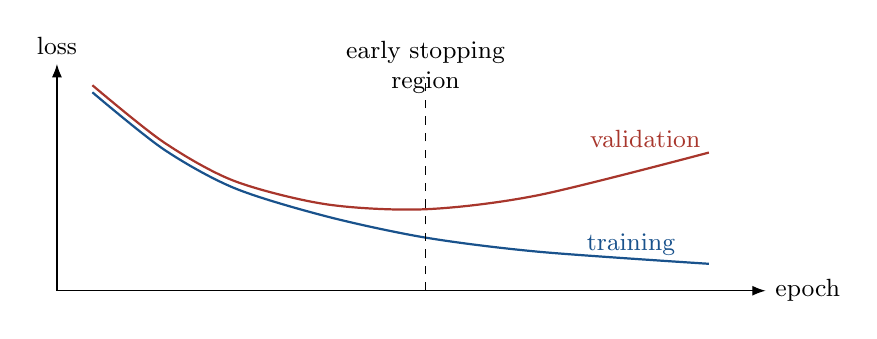
\begin{tikzpicture}[scale=0.9,>=Latex,every node/.style={font=\small}]
\draw[->] (0,0) -- (10,0) node[right] {epoch};
\draw[->] (0,0) -- (0,3.2) node[above] {loss};
\draw[fluidblue,thick] plot[smooth] coordinates {(0.5,2.8) (1.5,2.0) (2.5,1.45) (3.8,1.05) (5.2,0.75) (6.8,0.55) (9.2,0.38)};
\draw[fluidred,thick] plot[smooth] coordinates {(0.5,2.9) (1.5,2.1) (2.5,1.55) (3.8,1.22) (5.2,1.15) (6.8,1.35) (9.2,1.95)};
\draw[dashed] (5.2,0) -- (5.2,3.0);
\node[fluidblue] at (8.1,0.65) {training};
\node[fluidred] at (8.3,2.15) {validation};
\node[align=center] at (5.2,3.15) {early stopping\\region};
\end{tikzpicture}
\end{center}

Here ``epoch'' is the number of passes through the training data.  Training loss often decreases continuously, but validation loss can increase after overfitting begins.

% ============================================================
\section{Normalization and nondimensionalization}

Neural networks train better when inputs and targets have reasonable scales.  In fluids, scaling has two meanings: statistical normalization and physical nondimensionalization.

\subsection{Statistical normalization}

Standardization of a scalar feature is
\begin{equation}
    x_{\rm std}=\frac{x-\mu_x}{\sigma_x}.
    \label{eq:standardization}
\end{equation}
Here $x$ is the original scalar feature, $\mu_x$ is the mean of that feature in the training set, $\sigma_x$ is the standard deviation of that feature in the training set, and $x_{\rm std}$ is the standardized feature.

Min-max scaling is
\begin{equation}
    x_{\rm mm}=\frac{x-x_{\min}}{x_{\max}-x_{\min}}.
    \label{eq:minmax}
\end{equation}
Here $x$ is the original scalar feature, $x_{\min}$ is the minimum training-set value, $x_{\max}$ is the maximum training-set value, and $x_{\rm mm}$ is the min-max scaled feature.

\subsection{Physical nondimensionalization}

The Reynolds number is
\begin{equation}
    \re=\frac{\rho U L}{\mu}=\frac{U L}{\nu}.
    \label{eq:reynolds}
\end{equation}
Here $\re$ is the Reynolds number, $\rho$ is density, $U$ is a characteristic velocity, $L$ is a characteristic length, $\mu$ is dynamic viscosity, and $\nu=\mu/\rho$ is kinematic viscosity.

The Knudsen number is
\begin{equation}
    \kn=\frac{\lambda}{L}.
    \label{eq:knudsen}
\end{equation}
Here $\kn$ is the Knudsen number, $\lambda$ is the molecular mean free path, and $L$ is a characteristic macroscopic length.

The Mach number is
\begin{equation}
    \ma=\frac{U}{a}.
    \label{eq:mach}
\end{equation}
Here $\ma$ is the Mach number, $U$ is a characteristic flow velocity, and $a$ is the speed of sound.

\begin{keybox}{Practical rule for rarefied-flow ML}
Use physical nondimensional groups first, then apply statistical normalization to those groups.  For rarefied-flow datasets, use $\log_{10}\kn$ more often than $\kn$, because $\kn$ may span several orders of magnitude.
\end{keybox}

% ============================================================
\section{Rarefied-flow fundamentals for Week 2}

This course is not only about generic neural networks.  It is about neural networks for fluid dynamics, especially rarefied and non-equilibrium gas flows.  Therefore, students need the main rarefied-flow variables before building a surrogate.

\subsection{Mean free path}

The molecular mean free path is the average distance traveled by a molecule between collisions.  A common hard-sphere estimate is
\begin{equation}
    \lambda = \frac{k_B T}{\sqrt{2}\pi d^2 p}.
    \label{eq:mean_free_path}
\end{equation}
Here $\lambda$ is the mean free path, $k_B$ is Boltzmann's constant, $T$ is gas temperature, $d$ is the molecular diameter, and $p$ is gas pressure.

Equation~\eqref{eq:mean_free_path} shows that lower pressure increases $\lambda$.  Small devices also increase $\kn$ because $L$ becomes small in Eq.~\eqref{eq:knudsen}.

\subsection{Knudsen-number regimes}

A common regime classification is
\begin{center}
\begin{tabular}{p{0.22\linewidth}p{0.23\linewidth}p{0.43\linewidth}}
\toprule
Regime & Approximate range & Modeling implication \\
\midrule
Continuum & $\kn<10^{-3}$ & Navier-Stokes with no-slip walls is often appropriate. \\
Slip & $10^{-3}\le \kn<10^{-1}$ & Continuum equations may work with velocity-slip and temperature-jump boundary conditions. \\
Transition & $10^{-1}\le \kn<10$ & Strong non-equilibrium effects; DSMC, Boltzmann-type, BGK, or Fokker-Planck methods are often needed. \\
Free molecular & $\kn\ge 10$ & Molecule-wall interactions dominate over molecule-molecule collisions. \\
\bottomrule
\end{tabular}
\end{center}

Here $\kn$ is the Knudsen number defined in Eq.~\eqref{eq:knudsen}.  The boundaries between regimes are approximate; real model validity depends on geometry, gradients, Mach number, and wall physics.

\begin{center}
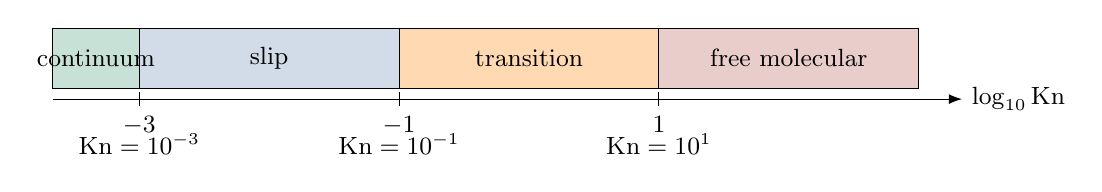
\begin{tikzpicture}[xscale=1.1,yscale=0.9,>=Latex,every node/.style={font=\small}]
\draw[->] (0,0) -- (10.5,0) node[right] {$\log_{10}\kn$};
\foreach \x/\lab in {1/$-3$,4/$-1$,7/$1$}{\draw (\x,0.1)--(\x,-0.1) node[below] {\lab};}
\fill[fluidgreen!25] (0,0.15) rectangle (1,1.0);
\fill[fluidblue!20] (1,0.15) rectangle (4,1.0);
\fill[orange!30] (4,0.15) rectangle (7,1.0);
\fill[fluidred!25] (7,0.15) rectangle (10,1.0);
\draw (0,0.15) rectangle (10,1.0);
\draw (1,0.15)--(1,1.0); \draw (4,0.15)--(4,1.0); \draw (7,0.15)--(7,1.0);
\node at (0.5,0.58) {continuum};
\node at (2.5,0.58) {slip};
\node at (5.5,0.58) {transition};
\node at (8.5,0.58) {free molecular};
\node[below] at (1,-0.35) {$\kn=10^{-3}$};
\node[below] at (4,-0.35) {$\kn=10^{-1}$};
\node[below] at (7,-0.35) {$\kn=10^{1}$};
\end{tikzpicture}
\end{center}

\subsection{Reynolds number versus Knudsen number}

The Reynolds number in Eq.~\eqref{eq:reynolds} compares inertia to viscous diffusion.  The Knudsen number in Eq.~\eqref{eq:knudsen} compares molecular length scale to device length scale.  They answer different questions.

\begin{center}
\begin{tabular}{p{0.22\linewidth}p{0.34\linewidth}p{0.34\linewidth}}
\toprule
Number & Measures & Main question \\
\midrule
$\re$ & inertia relative to viscosity & Is the flow dominated by inertia, viscosity, instability, or turbulence? \\
$\kn$ & molecular mean free path relative to geometry & Is the continuum assumption valid? \\
$\ma$ & flow speed relative to sound speed & Is compressibility important? \\
\bottomrule
\end{tabular}
\end{center}

\subsection{Velocity slip}

At a no-slip continuum wall,
\begin{equation}
    u_{\rm gas}|_w = u_w.
    \label{eq:no_slip}
\end{equation}
Here $u_{\rm gas}|_w$ is the gas tangential velocity evaluated at the wall, and $u_w$ is the wall tangential velocity.

In rarefied flow, a simplified first-order slip relation is
\begin{equation}
    u_{\rm slip}=u_{\rm gas}|_w-u_w \approx C_u\lambda\left.\frac{\partial u_t}{\partial n}\right|_w.
    \label{eq:slip}
\end{equation}
Here $u_{\rm slip}$ is the slip velocity, $u_{\rm gas}|_w$ is gas tangential velocity at the wall, $u_w$ is wall tangential velocity, $C_u$ is a slip coefficient depending on gas-surface interaction, $\lambda$ is mean free path, $u_t$ is tangential gas velocity, $n$ is the wall-normal coordinate, and $|_w$ indicates evaluation at the wall.

\subsection{Temperature jump}

At a continuum isothermal wall,
\begin{equation}
    T_{\rm gas}|_w = T_w.
    \label{eq:no_jump}
\end{equation}
Here $T_{\rm gas}|_w$ is the gas temperature at the wall and $T_w$ is the wall temperature.

In rarefied flow, a simplified temperature-jump relation is
\begin{equation}
    T_{\rm gas}|_w-T_w \approx C_T\lambda\left.\frac{\partial T}{\partial n}\right|_w.
    \label{eq:temperature_jump}
\end{equation}
Here $T_{\rm gas}|_w-T_w$ is the temperature jump, $C_T$ is a temperature-jump coefficient, $\lambda$ is mean free path, $T$ is gas temperature, $n$ is the wall-normal coordinate, and $|_w$ indicates wall evaluation.

\subsection{Accommodation coefficient}

The accommodation coefficient $\alpha$ measures how strongly gas molecules equilibrate with a surface.  In simplified terms:
\begin{itemize}
    \item $\alpha\approx1$ means strong accommodation, often associated with diffuse-like reflection;
    \item $\alpha<1$ means partial accommodation and more memory of incoming molecular velocity.
\end{itemize}

Accommodation affects slip, temperature jump, and energy exchange at walls.  Therefore, it is a natural feature in rarefied-flow machine-learning datasets.

\subsection{Knudsen layer}

A Knudsen layer is a near-wall non-equilibrium region with thickness on the order of a few mean free paths.  Inside this layer, continuum constitutive laws may not accurately describe stress and heat flux.

For ML, the important message is: a model can have low global error but still fail near the wall.  Therefore, wall error and near-wall validation are important.

% ============================================================
\section{Neural-network surrogate for a rarefied-flow quantity}

The Week-2 coding lab uses a synthetic rarefied-flow relation.  It is not a replacement for DSMC or experiments.  It is a controlled teaching problem where the true function is known.

The input feature vector is
\begin{equation}
    \bx = \begin{bmatrix} r \\ \alpha \\ \Pi \\ \Theta \end{bmatrix},
    \qquad r=\log_{10}\kn, \qquad \Pi=\frac{p_{\rm in}}{p_{\rm out}}, \qquad \Theta=\frac{T_w}{T_0}.
    \label{eq:lab_features}
\end{equation}
Here $\bx$ is the feature vector, $r$ is the logarithmic Knudsen-number feature, $\kn$ is Knudsen number, $\alpha$ is accommodation coefficient, $\Pi$ is inlet-to-outlet pressure ratio, $p_{\rm in}$ is inlet pressure, $p_{\rm out}$ is outlet pressure, $\Theta$ is wall-to-reference temperature ratio, $T_w$ is wall temperature, and $T_0$ is reference temperature.

A synthetic normalized mass-flow proxy is
\begin{equation}
    Q^* = \left(1-\frac{1}{\Pi}\right)
    \left[1 + C_s\frac{2-\alpha}{\alpha}\frac{\kn}{1+\kn}\right]
    \Theta^{-1/2}
    \left[1+C_r\tanh\left(\log_{10}\kn+1\right)\right]
    +\eps.
    \label{eq:synthetic_Q}
\end{equation}
Here $Q^*$ is the synthetic nondimensional mass-flow proxy, $\Pi$ is pressure ratio, $C_s$ is a chosen slip-strength coefficient, $\alpha$ is accommodation coefficient, $\kn$ is Knudsen number, $\Theta$ is temperature ratio, $C_r$ is a chosen rarefaction-transition coefficient, $\tanh$ is the hyperbolic tangent function, and $\eps$ is a small noise term representing numerical or measurement noise.

The neural network approximates
\begin{equation}
    \widehat{Q}^* = f_{\btheta}(r,\alpha,\Pi,\Theta).
    \label{eq:network_Q}
\end{equation}
Here $\widehat{Q}^*$ is the predicted normalized mass-flow proxy, $f_{\btheta}$ is the neural-network model, $\btheta$ denotes all weights and biases, and $r$, $\alpha$, $\Pi$, and $\Theta$ are features defined in Eq.~\eqref{eq:lab_features}.

\subsection{Why compare with baselines?}

A neural network should not be accepted just because it is nonlinear.  It should be compared with simple baselines:
\begin{itemize}
    \item a constant mean predictor;
    \item polynomial regression;
    \item interpolation or nearest-neighbor prediction;
    \item a simple physical scaling relation.
\end{itemize}

If a DNN does not outperform these baselines, the DNN is not useful for that task.

% ============================================================
\section{Physical validation checks for Week 2}

For the synthetic $Q^*$ model in Eq.~\eqref{eq:synthetic_Q}, useful checks include:

\subsection{Positivity check}

A mass-flow proxy should not be negative in the selected parameter range:
\begin{equation}
    \widehat{Q}^* \ge 0.
    \label{eq:positivity_check}
\end{equation}
Here $\widehat{Q}^*$ is the DNN-predicted normalized mass-flow proxy.

\subsection{Pressure-ratio monotonicity check}

For fixed $\kn$, $\alpha$, and $\Theta$, increasing $\Pi$ should increase the driving pressure effect in Eq.~\eqref{eq:synthetic_Q}.  A discrete check is
\begin{equation}
    \widehat{Q}^*(\Pi_2)-\widehat{Q}^*(\Pi_1) \ge 0 \quad \text{for} \quad \Pi_2>\Pi_1.
    \label{eq:monotonicity_check}
\end{equation}
Here $\widehat{Q}^*(\Pi_1)$ and $\widehat{Q}^*(\Pi_2)$ are DNN predictions at pressure ratios $\Pi_1$ and $\Pi_2$, with all other features fixed.

\subsection{Regime-wise error}

Compute separate errors in each Knudsen regime:
\begin{equation}
    \rmse_{\mathcal{R}} = \sqrt{\frac{1}{N_{\mathcal{R}}}\sum_{i\in\mathcal{R}}\left(Q^{*(i)}-\widehat{Q}^{*(i)}\right)^2}.
    \label{eq:regime_rmse}
\end{equation}
Here $\rmse_{\mathcal{R}}$ is the root-mean-squared error in regime $\mathcal{R}$, $N_{\mathcal{R}}$ is the number of samples in that regime, $i$ is a sample index in the regime, $Q^{*(i)}$ is the true synthetic value, and $\widehat{Q}^{*(i)}$ is the predicted value.

A model can have acceptable total RMSE while failing badly in the transition regime.  Regime-wise reporting is therefore essential.

\subsection{Extrapolation check}

If training uses only
\begin{equation}
    -3\le \log_{10}\kn \le -1,
    \label{eq:train_kn_range}
\end{equation}
where $\kn$ is Knudsen number, then predictions at $\log_{10}\kn> -1$ are extrapolations into transition or free-molecular regimes.  A DNN may return smooth outputs there, but smoothness is not physical validity.

% ============================================================
\section{How the Week-2 Colab matches this lecture}

The Colab notebook follows this sequence:
\begin{enumerate}
    \item build one-neuron predictions by hand;
    \item plot activation functions;
    \item demonstrate one gradient-descent update;
    \item generate the synthetic rarefied-flow dataset from Eq.~\eqref{eq:synthetic_Q};
    \item classify samples by $\kn$ regime;
    \item split data into training, validation, and test sets;
    \item train polynomial-regression and nearest-neighbor baselines;
    \item train a small DNN;
    \item compare errors inside and outside the training range;
    \item perform physical validation checks.
\end{enumerate}

\begin{lstlisting}[language=Python,caption={Typical Keras model for the Week-2 lab.}]
model = keras.Sequential([
    layers.Input(shape=(4,)),
    layers.Dense(32, activation="tanh"),
    layers.Dense(32, activation="tanh"),
    layers.Dense(1, activation="linear")
])
model.compile(optimizer=keras.optimizers.Adam(learning_rate=1e-3),
              loss="mse",
              metrics=["mae"])
\end{lstlisting}

In this code, the input dimension is $4$ because the features are $r=\log_{10}\kn$, $\alpha$, $\Pi$, and $\Theta$.  The two hidden layers each contain $32$ neurons.  The output layer has one neuron because the target is the scalar $Q^*$.  The linear output activation is used because this is a regression problem.

% ============================================================
\section{Common student mistakes}

\begin{warnbox}{Mistake 1: Treating the DNN as magic}
A DNN is a parameterized function.  It maps inputs to outputs.  It does not know conservation laws, wall physics, or regime boundaries unless those are represented in the data, features, loss, architecture, or validation.
\end{warnbox}

\begin{warnbox}{Mistake 2: Training and testing on the same data}
If the same samples are used for training and testing, the reported error is not a meaningful measure of generalization.
\end{warnbox}

\begin{warnbox}{Mistake 3: Scaling the test set using test statistics}
Scalers must be fit on the training set only.  Then the same scaling transformation is applied to validation and test data.
\end{warnbox}

\begin{warnbox}{Mistake 4: Ignoring extrapolation}
A random split may hide extrapolation problems.  For rarefied flows, deliberately test outside the training $\kn$ range to see whether the model is robust.
\end{warnbox}

\begin{warnbox}{Mistake 5: Reporting only one number}
A single RMSE value is not enough.  Report baseline comparisons, regime-wise errors, physical checks, and limitations.
\end{warnbox}

% ============================================================
\section{Study questions}

Students should be able to answer the following without looking at code:
\begin{enumerate}
    \item What are the features and target in the Week-2 rarefied-flow surrogate?
    \item In $z=\bm{w}^T\bx+b$, what are $z$, $\bm{w}$, $\bx$, and $b$?
    \item Why is a bias needed in a neuron?
    \item Why does a neural network need activation functions?
    \item What is the difference between regression and classification?
    \item What does the learning rate control?
    \item What does backpropagation compute?
    \item Why can training loss decrease while validation loss increases?
    \item Why is $\log_{10}\kn$ often a better feature than $\kn$?
    \item Why is extrapolation from the slip regime to the transition regime risky?
    \item What two physical checks would you apply to a rarefied mass-flow surrogate?
    \item Why should every DNN be compared against a simpler baseline?
\end{enumerate}

% ============================================================
\section{Summary}

A neural network is a trainable nonlinear function.  It is built from neurons, and each neuron computes a weighted sum, adds a bias, and passes the result through an activation function.  Learning means changing the weights and biases to reduce a loss function.  Backpropagation computes the gradients needed for this learning process.

For AI in fluids, the network is only one part of the workflow.  The full workflow includes physical nondimensionalization, feature design, train/validation/test splitting, baseline comparison, numerical error metrics, and physical validation.  In rarefied flows, the most important physical feature is often the Knudsen number, because it indicates when continuum assumptions weaken and kinetic effects become important.

\begin{keybox}{Final message of Week 2}
A useful neural-network surrogate is not the one with the lowest training loss.  A useful surrogate is the one that predicts accurately, beats simple baselines, respects known physical behavior, and clearly states where it is likely to fail.
\end{keybox}

% ============================================================
\section*{References and supporting materials}
\begin{enumerate}
    \item J. Nathan Kutz, \emph{Data-Driven Modeling \& Scientific Computation: Methods for Integrating Dynamics of Complex Systems and Big Data}, second-edition course manuscript.
    \item E. Roohi, H. Akhlaghi, and S. Stefanov, \emph{Advances in Direct Simulation Monte Carlo: From Micro-Scale to Rarefied Flow Phenomena}, Springer Nature, 2025.
    \item G. A. Bird, \emph{Molecular Gas Dynamics and the Direct Simulation of Gas Flows}, Oxford University Press, 1994.
    \item C. Cercignani, \emph{Rarefied Gas Dynamics: From Basic Concepts to Actual Calculations}, Cambridge University Press, 2000.
    \item S. Mirjalili, neural-network lecture set used as supporting teaching material: analogy, neuron model, terminology, learning in neural networks, cost functions, activation functions, multi-layer perceptron, deep neural networks, backpropagation, momentum, and regression using MLPs.
\end{enumerate}

\end{document}
